% **************************************************
% Document Class Definition
% **************************************************
\documentclass[%
	paper=A4,					% paper size --> A4 is default in Germany
	twoside=true,				% onesite or twoside printing
	openright,					% doublepage cleaning ends up right side
	parskip=full,				% spacing value / method for paragraphs
	chapterprefix=true,			% prefix for chapter marks
	11pt,						% font size
	headings=normal,			% size of headings
	bibliography=totoc,			% include bib in toc
	listof=totoc,				% include listof entries in toc
	titlepage=on,				% own page for each title page
	captions=tableabove,		% display table captions above the float env
	draft=true,				% value for draft version
]{scrreprt}%

% **************************************************
% Debug LaTeX Information
% **************************************************
%\listfiles

% **************************************************
% Information and Commands for Reuse
% **************************************************
\newcommand{\thesisTitle}{Mixed Reality Media: Integration of live video feed in 3D environments}
\newcommand{\thesisName}{Martin Zier}
\newcommand{\thesisSubject}{Bachelor Thesis}
\newcommand{\thesisDate}{\today}
\newcommand{\thesisVersion}{Initial Drafting}

\newcommand{\thesisFirstReviewer}{Kristian Hildebrand}
\newcommand{\thesisFirstReviewerUniversity}{\protect{Beuth University of Applied Sciences}}
\newcommand{\thesisFirstReviewerDepartment}{Department VI: Computer Sciences and Media}

\newcommand{\thesisSecondReviewer}{Prof. Dr.-Ing. Ren\'e G\"orlich}
\newcommand{\thesisSecondReviewerUniversity}{\protect{Beuth University of Applied Sciences}}
\newcommand{\thesisSecondReviewerDepartment}{Department VI: Computer Sciences and Media}

\newcommand{\thesisFirstSupervisor}{Kristian Hildebrand}
\newcommand{\thesisSecondSupervisor}{Joachim Quantz}

\newcommand{\thesisUniversity}{\protect{Beuth University of Applied Sciences}}
\newcommand{\thesisUniversityDepartment}{Department VI: Computer Sciences and Media}
\newcommand{\thesisUniversityInstitute}{ }
\newcommand{\thesisUniversityGroup}{ }
\newcommand{\thesisUniversityCity}{Berlin}
\newcommand{\thesisUniversityStreetAddress}{Luxemburger Stra{\ss}e 10}
\newcommand{\thesisUniversityPostalCode}{13353}

% **************************************************
% Load and Configure Packages
% **************************************************
\usepackage[utf8]{inputenc}		% defines file's character encoding
\usepackage[english]{babel} % babel system, adjust the language of the content
\usepackage[					% clean thesis style
	figuresep=colon,%
	sansserif=false,%
	hangfigurecaption=false,%
	hangsection=true,%
	hangsubsection=true,%
	colorize=full,%
	colortheme=bluemagenta,%
	bibsys=bibtex,%
	bibfile=bib-refs,%
	bibstyle=alphabetic,%
]{cleanthesis}

\usepackage{todonotes}
\usepackage{listings}


\hypersetup{					% setup the hyperref-package options
	pdftitle={\thesisTitle},	% 	- title (PDF meta)
	pdfsubject={\thesisSubject},% 	- subject (PDF meta)
	pdfauthor={\thesisName},	% 	- author (PDF meta)
	plainpages=false,			% 	-
	colorlinks=false,			% 	- colorize links?
	pdfborder={0 0 0},			% 	-
	breaklinks=true,			% 	- allow line break inside links
	bookmarksnumbered=true,		%
	bookmarksopen=true			%
}

% **************************************************
% Document CONTENT
% **************************************************
\begin{document}

% --------------------------
% rename document parts
% --------------------------
%\renewcaptionname{ngerman}{\figurename}{Abb.}
%\renewcaptionname{ngerman}{\tablename}{Tab.}
\renewcaptionname{english}{\figurename}{Fig.}
\renewcaptionname{english}{\tablename}{Tab.}

% --------------------------
% Front matter
% --------------------------
\pagenumbering{roman}			% roman page numbing (invisible for empty page style)
\pagestyle{empty}				% no header or footers
% !TEX root = ../thesis-example.tex
% ------------------------------------  --> main title page
\begin{titlepage}
	\pdfbookmark[0]{Titlepage}{Titlepage}
	\tgherosfont
	\centering

	
\includegraphics[width=12cm]{_external/media/Beuth-Logo.png} \\[2mm]
	\textsf{\thesisUniversityDepartment} \\
	\textsf{\thesisUniversityInstitute} \\
	\textsf{\thesisUniversityGroup} \\

	\vfill
	{\large \thesisSubject} \\[5mm]
	{\LARGE \color{ctcolortitle}\textbf{\thesisTitle} \\[10mm]}
	{\Large \thesisName} \\

	\vfill
	\begin{minipage}[t]{.27\textwidth}
		\raggedleft
		\textit{1. Reviewer}
	\end{minipage}
	\hspace*{15pt}
	\begin{minipage}[t]{.65\textwidth}
		{\Large \thesisFirstReviewer} \\
	  	{\small \thesisFirstReviewerDepartment} \\[-1mm]
		{\small \thesisFirstReviewerUniversity}
	\end{minipage} \\[5mm]
	\begin{minipage}[t]{.27\textwidth}
		\raggedleft
		\textit{2. Reviewer}
	\end{minipage}
	\hspace*{15pt}
	\begin{minipage}[t]{.65\textwidth}
		{\Large \thesisSecondReviewer} \\
	  	{\small \thesisSecondReviewerDepartment} \\[-1mm]
		{\small \thesisSecondReviewerUniversity}
	\end{minipage} \\[10mm]
	\begin{minipage}[t]{.27\textwidth}
		\raggedleft
		\textit{Supervisor}
	\end{minipage}
	\hspace*{15pt}
	\begin{minipage}[t]{.65\textwidth}
		\thesisFirstSupervisor\
	\end{minipage} \\[10mm]

	\thesisDate \\

\end{titlepage}


% ------------------------------------  --> lower title back for single page layout
\hfill
\vfill
{
	\small
	\textbf{\thesisName} \\
	\textit{\thesisTitle} \\
	\thesisSubject, \thesisDate \\
	Reviewers: \thesisFirstReviewer\ and \thesisSecondReviewer \\
	Supervisor: \thesisFirstSupervisor \\[1.5em]
	\textbf{\thesisUniversity} \\
%	\textit{\thesisUniversityGroup} \\
%	\thesisUniversityInstitute \\
	\thesisUniversityDepartment \\
	\thesisUniversityStreetAddress \\
	\thesisUniversityPostalCode\ \thesisUniversityCity
}
		% INCLUDE: all titlepages
\cleardoublepage

\pagestyle{plain}				% display just page numbers
% !TeX spellcheck = en_US
% !TEX root = ../thesis-example.tex
%
\pdfbookmark[0]{Abstract}{Abstract}
\chapter*{Abstract}
\label{sec:abstract}
\vspace*{-10mm}

Virtual Reality is no distance dream anymore, but the technology has a 
marketing problem: A view through the eyes of the head-mounted display wearer 
is bland and loses the usage context. Following the first-person view is hard 
and it shows twitchy, unnatural motion.

This thesis discusses a general rendering pipeline for runtime 3D engines for 
Mixed Reality Media, a form of video composition that places a real person 
inside a virtual reality scene. The real world video will be augmented by 
multiple video techniques and parameters from the virtual environment.
\newline
For example this allows for recreation of light conditions from the virtual 
scene and creates an immersive and inviting view into the virtual scenery.

\begin{center}
	\hrulefill
\end{center}

VR ist kein entfernter Traum mehr, doch die Technologie hat ein 
Marketing-Problem: Ein Blick durch die Augen des Headset-Trägers ist 
uninteressant und verliert den Nutzerkontext. Der First-Person Sicht ist nur 
schwer zu folgen und zeigt unruhige, unnatürliche Bewegungen.

Diese Bachelor Arbeit beschäftigt sich mit dem Aufbau einer allgemeinen Mixed 
Reality Pipeline für Echtzeit 3D Engines, eine Aufarbeitung von 
Echtbildaufnahmen eines VR Nutzers und die Rückführung in eine virtuelle Szene. 
Durch mehrere Videoverfahren wird das Bild des Trägers mit der virtuellen Welt 
zusammengeführt und mit den Parametern der virtuellen Welt erweitert.
\newline
Dadurch können z. B. Lichtverhältnisse der virtuellen Szenerie nachempfunden 
werden und einen immersiven und einladenden Blick in den virtuellen Raum 
geboten werden.		% INCLUDE: the abstracts (english and german)
\cleardoublepage
%
% !TeX spellcheck = en_US
% !TEX root = ../thesis-example.tex
%
\pdfbookmark[0]{Acknowledgement}{Acknowledgement}
\chapter*{Acknowledgement}
\label{sec:acknowledgement}
\vspace*{-10mm}

This thesis is dedicated to background noise: 

Background noise! Background noise makes nothing easier - get it now from your 
local certified background noise dealer.
 % INCLUDE: acknowledgement
\cleardoublepage
%
\setcounter{tocdepth}{2}		% define depth of toc
\tableofcontents				% display table of contents
\cleardoublepage

% --------------------------
% Body matter
% --------------------------
\pagenumbering{arabic}			% arabic page numbering
\setcounter{page}{1}			% set page counter
\pagestyle{maincontentstyle} 	% fancy header and footer

% !TeX spellcheck = en_US
% !TEX root = ../thesis-example.tex
%
\chapter{Introduction}
\label{sec:intro}

\cleanchapterquote{If a technological feat is possible, man will do it. Almost 
as if it's wired into the core of our being.}{Motoko Kusanagi}{(Ghost in the 
Shell)}

Extending reality with the help of computer generated imagery is no new 
concept. Ever since real time 3D graphics was possible there was an attempt to 
extend the understanding of reality. Within the recent years there have been 
great successes in the industry, most notably in image augmentation was 
"Pokémon Go" with an estimated install base of 750 million downloads 
worldwide in June, 2017. \cite{appannie:2017}  Just before this thesis 
started, Apple and Google showed off their consumer-ready hard- and software 
for augmented reality experiences.
\newline
Virtual Reality Head Mounted Displays have had a similar push in sales with an 
approximate of 5.83 million sold devices, which range in a sales price between 
80 - 900€ for a VR kit, ranging from the very simple Google Daydream View and 
the very sophisticated HTC Vive. \cite{erguerel:2017} And in these figures are 
the sales of Google Cardboards missing, which is approximated at around 80 
Million.
\newline
This generation of computer systems, which includes PC workstations, game 
consoles and smartphones, is finally sophisticated enough in computation speed 
and sensor-sensitivity to allow low latency tracking, precise to just a few 
millimeters spanning over an area of about $35m^2$.

\section{Overview}
\label{sec:intro:outline}

The idea of Virtual Reality (VR) and Head Mounted Displays (HMDs) stems from a 
cultural need to slip into roles of foreign worlds. Through the advancing 
development of hard- and software over the last decades emerges a medium which 
has unmatched immersion and creates an unique, transforming experience into any 
imaginable environment.

VR and HMDs are now advanced enough for consumer markets - but it stumbles at 
communicating the experience. Without having ever put on a VR-Headset it is 
nearly impossible to understand - or even imagine - what the virtual reality 
experience means. Any observer of VR, usually done by showing what 
the VR actor is seeing, will not be able to get an understanding of the 
importance and shift of reality perception without wearing the headset himself.
\newline
Showing the video output from a HMD as marketing material is contradicting with 
classic motion video productions. There is even only one famous example where 
the perspective of a First Person Shooter is reenacted, which was in the 
overwhelmingly negatively received Doom (2005) movie.

The VR industry, including but not limited to game developers, exhibition 
creators and creative studios is in need of better communication of their 
products that includes more than the current headset wearer and allows for a 
similar, immersive but adapted experience.
\newline
The currently next step is called "Mixed Reality" (MR) and uses an external 
camera with the same tracking hardware of the headset to produce a video signal 
that shows the real world actor with the environment around him. There are 
currently three main ways of producing MR footage - where as only one variant 
allows for live compositing with highly accurate imaging results, which will be 
discussed in this thesis.

\section{Motivation}
\label{sec:intro:motivation}

My early teenage years started around the time where digitalization and global
interconnectivity begun and broadband Internet became commercially available.
Suddenly remote multiplayer games, unlimited image sharing - and yes, music
sharing, too -, Java-Applets, Flash, HTML framesets and "Marquee" CSS emerged in
that medium. 3D Acceleration became a de-facto standard and even simple office
PCs got weak, but dedicated graphics processing units built in. The mass of
pixels by increasing the resolution of displays was basically a yearly
iteration in greater, better, smaller, denser and brighter.

I am personally very interested and invested in Virtual/Mixed/Augmented Reality 
to succeed and liked the idea to merge multiple forms of media into one - which 
is, in my personal opinion, a great summary of my studies and its contents. 
This thesis represents my interests and the reasons why I chose these studies.

\section{Problem Statement}
\label{sec:intro:problem}

Initially I will research motion video productions, computer generated imagery 
and color theory. This leads to the knowledge of implementing basic, 
interactive live motion video feeds.
\newline
The core aspect will be integrating a multitude of Hardware in a software that 
allows for dynamic video compositing in 3D environments at runtime while a user 
is interacting with the virtual reality scene. This allows that the actor 
using the Vive HMD to be composited into the scenery from a third person view 
and it will looking like he is surrounded by the virtual scenery. The essential 
difference between classic post production is, that this system is planned to 
operate on runtime, allowing additional observers to get an interesting 
composited imagery of what the VR actor is experiencing.
\newline
An additional extension is to dynamically track the cameras position, allowing 
for dynamic camera movement and a freely moving actor. 

\section{Challenges \& Scope}
\label{sec:intro:challenges}

This thesis discusses the development and usage of a mixed reality setup inside 
a single PC and a single application.
\newline
It will highlight the core motion video production for mixed reality, as it 
differs from other MR setups, by staying inside the programs boundaries, 
integrating natively with the engine. Initially there is a need to solve for 
different input latencies, especially from the live video feed, which changes 
the rendering pipeline significantly.
\newline
Another core aspect will be chroma keying in real time rendering, as well as 
image reproduction from the chroma result. In detail there will be a discourse 
of layered image composition as result of fore- and background of the VR actor.
\newline
Lastly composition controls will be implemented, adding a color-correction 
layer to the input video, giving a more natural look to the actor inside a 
surrounding 3D environment.

Outside of the scope of this thesis will be green screen compositing, as it is 
used as tool - the same goes for video matting, which would require its own 
research for accurate realtime results with little to none user guidance. 
\cite{gong:realtime-matting:2010}, \cite{gastal:shared-sampling:2010}

\section{Results}
\label{sec:intro:results}

Result stuff

\section{Thesis Structure}
\label{sec:intro:structure}

This thesis gets contemplated by digital material hosted on GitHub. Print is a 
great medium, but lacks the ability for short demonstrations of video imaging 
solutions, problems and edge cases. To visualize these issues properly, all 
video media will have an annotation for cross referencing on the website. It is 
strongly suggested to follow these links for better understanding and 
highlighting of certain problems. They are be sorted by chapters for easier 
navigation.
% !TeX spellcheck = en_US
% !TEX root = ../thesis-example.tex
%
\chapter{Extending Reality}
\label{sec:extendingreality}

\cleanchapterquote{You are an aperture through which the universe is looking at 
and exploring itself.}{Alan W. Watts}{(Philosopher)}

The well known urban legend of "L'Arriv\'ee d'un train en gare de La Ciotat" in 
which a train arrives at the La Ciotat station, is, that "the audience was so 
overwhelmed by the moving image [...] coming directly at them that people 
screamed and ran to the back of the room". \cite{wiki:train:2017} With that a 
new medium was born, which matured into a new art form of film and movies.
\newline
Most important takeaway is, that with this short clip alone, a door beyond 
still images and their limited depiction of motion has been opened. Video 
imagery changed our imagination and allowed for a new communication form, 
inviting into an animated, moving world. There have been great achievements in 
the last century in motion video production with a great amount of visual 
trickery for composing more realistic and imaginative video content. With the 
help of Computer Generated Imagery (CGI) blurs the boundaries between real 
acting and virtual recreation so far, that it is almost impossible to 
differentiate between real world video capture and 3D recreated imagery in high 
budget productions.

\section{Motion Video Production}

Producing motion video has come a long way and a sufficient history of it would 
be far out of scope for this thesis. Concentrating on key aspects of 
composition techniques might give an appropriate overview to range where Mixed 
Reality takes its inspiration from.

Way before digital imaging processing took over production sets similar 
problems as discussed in this thesis had to be solved, in example how an actor 
can be captured without a back- or foreground and how he would then be 
integrated into an imaginative set. Today, modern action movies don't even 
necessarily capture the actor but his movements, which then will be 
artificially rendered with help of CGI. \todo{Missing: Camera tricks, computer 
aided visual effects, green screens}

\section{CGI \& Video Composition}

\subsection{History of Green \& Blue Screen Productions}

Set theory is beyond the scope of this thesis, but green- and blue screen 
production has first and foremost a simple reasoning: Green and blue are two of 
the three color triplets that resemble a least amount of color found in 
capturing of humans - and to a certain extent any flora or fauna. Since chroma 
keying (see Ch. \ref{sec:chromakey}) takes color distance as general basis, 
production environments use green screen keying in varying forms. Next to 
$\Delta E$, which will be discussed further, another approach is the 
calculation of fore- and background color spaces and separation of them. The 
latter solution is highly computation intense and is not suitable for runtime 
applications. \cite{disney:unmixing:2017}
\newline
Green boxes also abuse a correlating advantage that the human eye is most 
susceptible to green, allowing for a visual high color range and an ability to 
differentiate between many shades of green. Experiments to color range have 
been done since 1942, trying to understand gambit ranges and color 
differentiation of human vision. Experiments concluded that eye cone cells see 
a blending range of wavelengths to different intensities, giving the green 
vector space its highest perceptible range. \cite{MacAdam:1942}

\begin{figure}[htbp]
	\label{fig:greenscreen:stimula}
	\begin{subfigure}[t]{.35\textwidth}
		\centering
		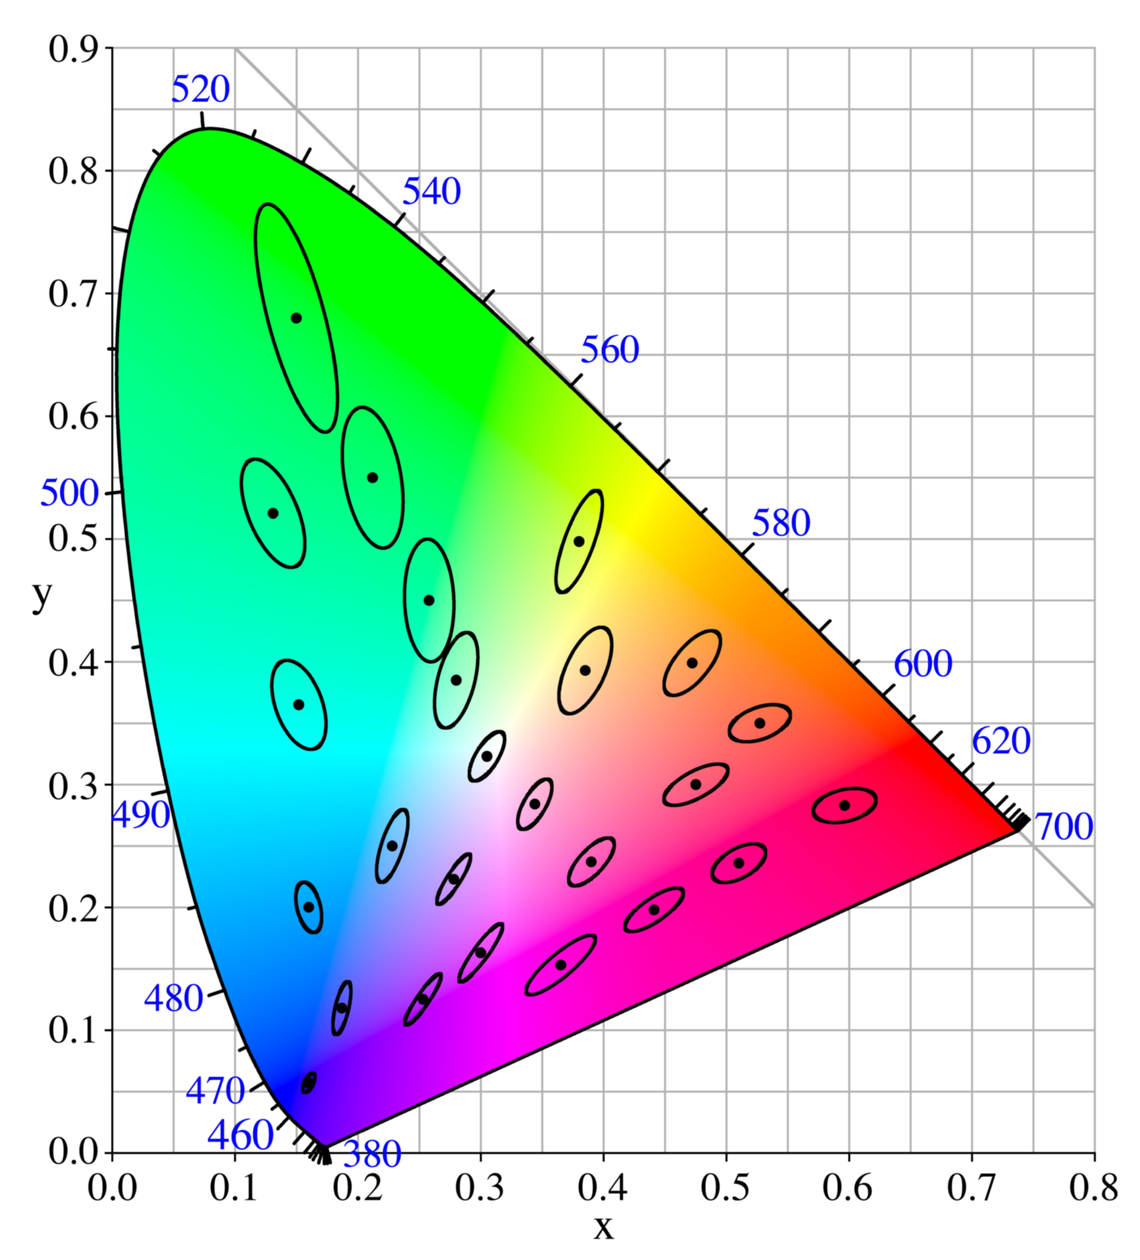
\includegraphics[width=\textwidth]{_external/media/CIExy1931_MacAdam.png}
	\caption{MacAdam ellipses on 1931 standard chromaticity diagram 
		\cite{wiki:macadam:2017}}
	\end{subfigure}
	\begin{subfigure}[t]{.5\textwidth}
		\centering
		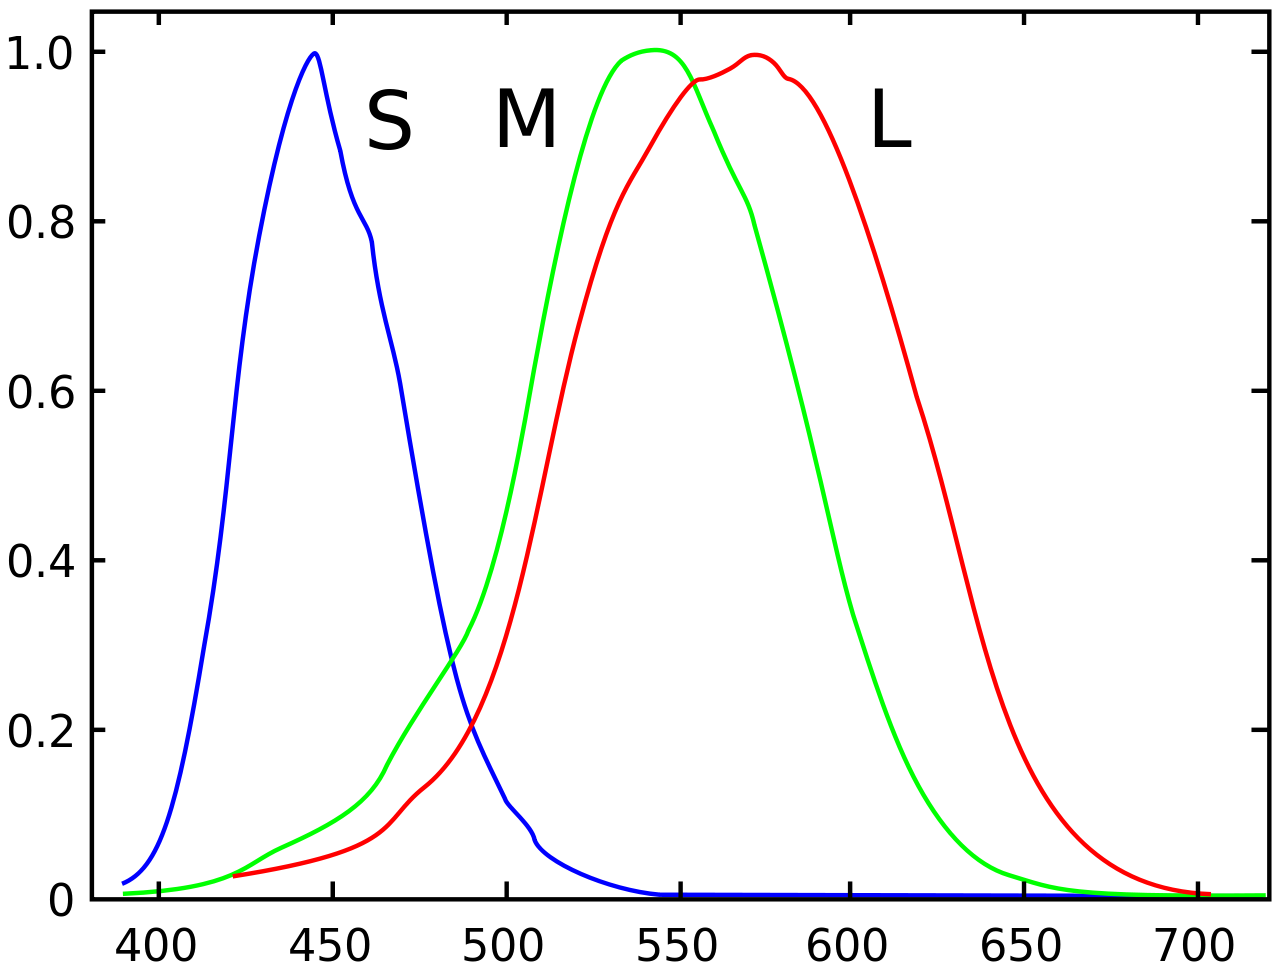
\includegraphics[width=\textwidth]{_external/media/1280px-Cones_SMJ2_E.png}
		\caption{Normalized responsivity spectra of human cone cells, S, M, and 
		L types after Wyszecki et. al \cite{wiki:Wyszecki:2017}}. Notice the 
		overlap between M and L cones.
	\end{subfigure}
\end{figure} \todo{The layout is a bit wonky here.}

Most consumer cameras - and even most production cameras - use dot-matrix 
sensors with a weighted ration of green (4), red (2) and blue (2) pixels, 
called Bayer pattern \cite{kodak:bayer:1976}, giving it - similar to human 
vision - a high color vector space. Green is generally easier to light, 
illuminate and adjust over blue screens. Small irregularities, for example 
through uneven lightning or crinkles in the material, can be adjusted easily by 
the user and allows for a relatively clean camera image generation.
\newline
The quality of input footage makes a big difference in separating back- and 
foreground, hence a well lit and adjusted set is a good backbone for well 
working chroma keying.

\section{What's VR - Differentiation of AR, VR \& MR}

In search of an appropriate abbreviation for computer-enhanced real time 
imagery a recent addition is "XR", where \textit{X} is a letter of your choice. 
Definitions are getting more diluted and generally describe a technique, rather 
than an apparent effect by now.

\begin{figure}[htb]
	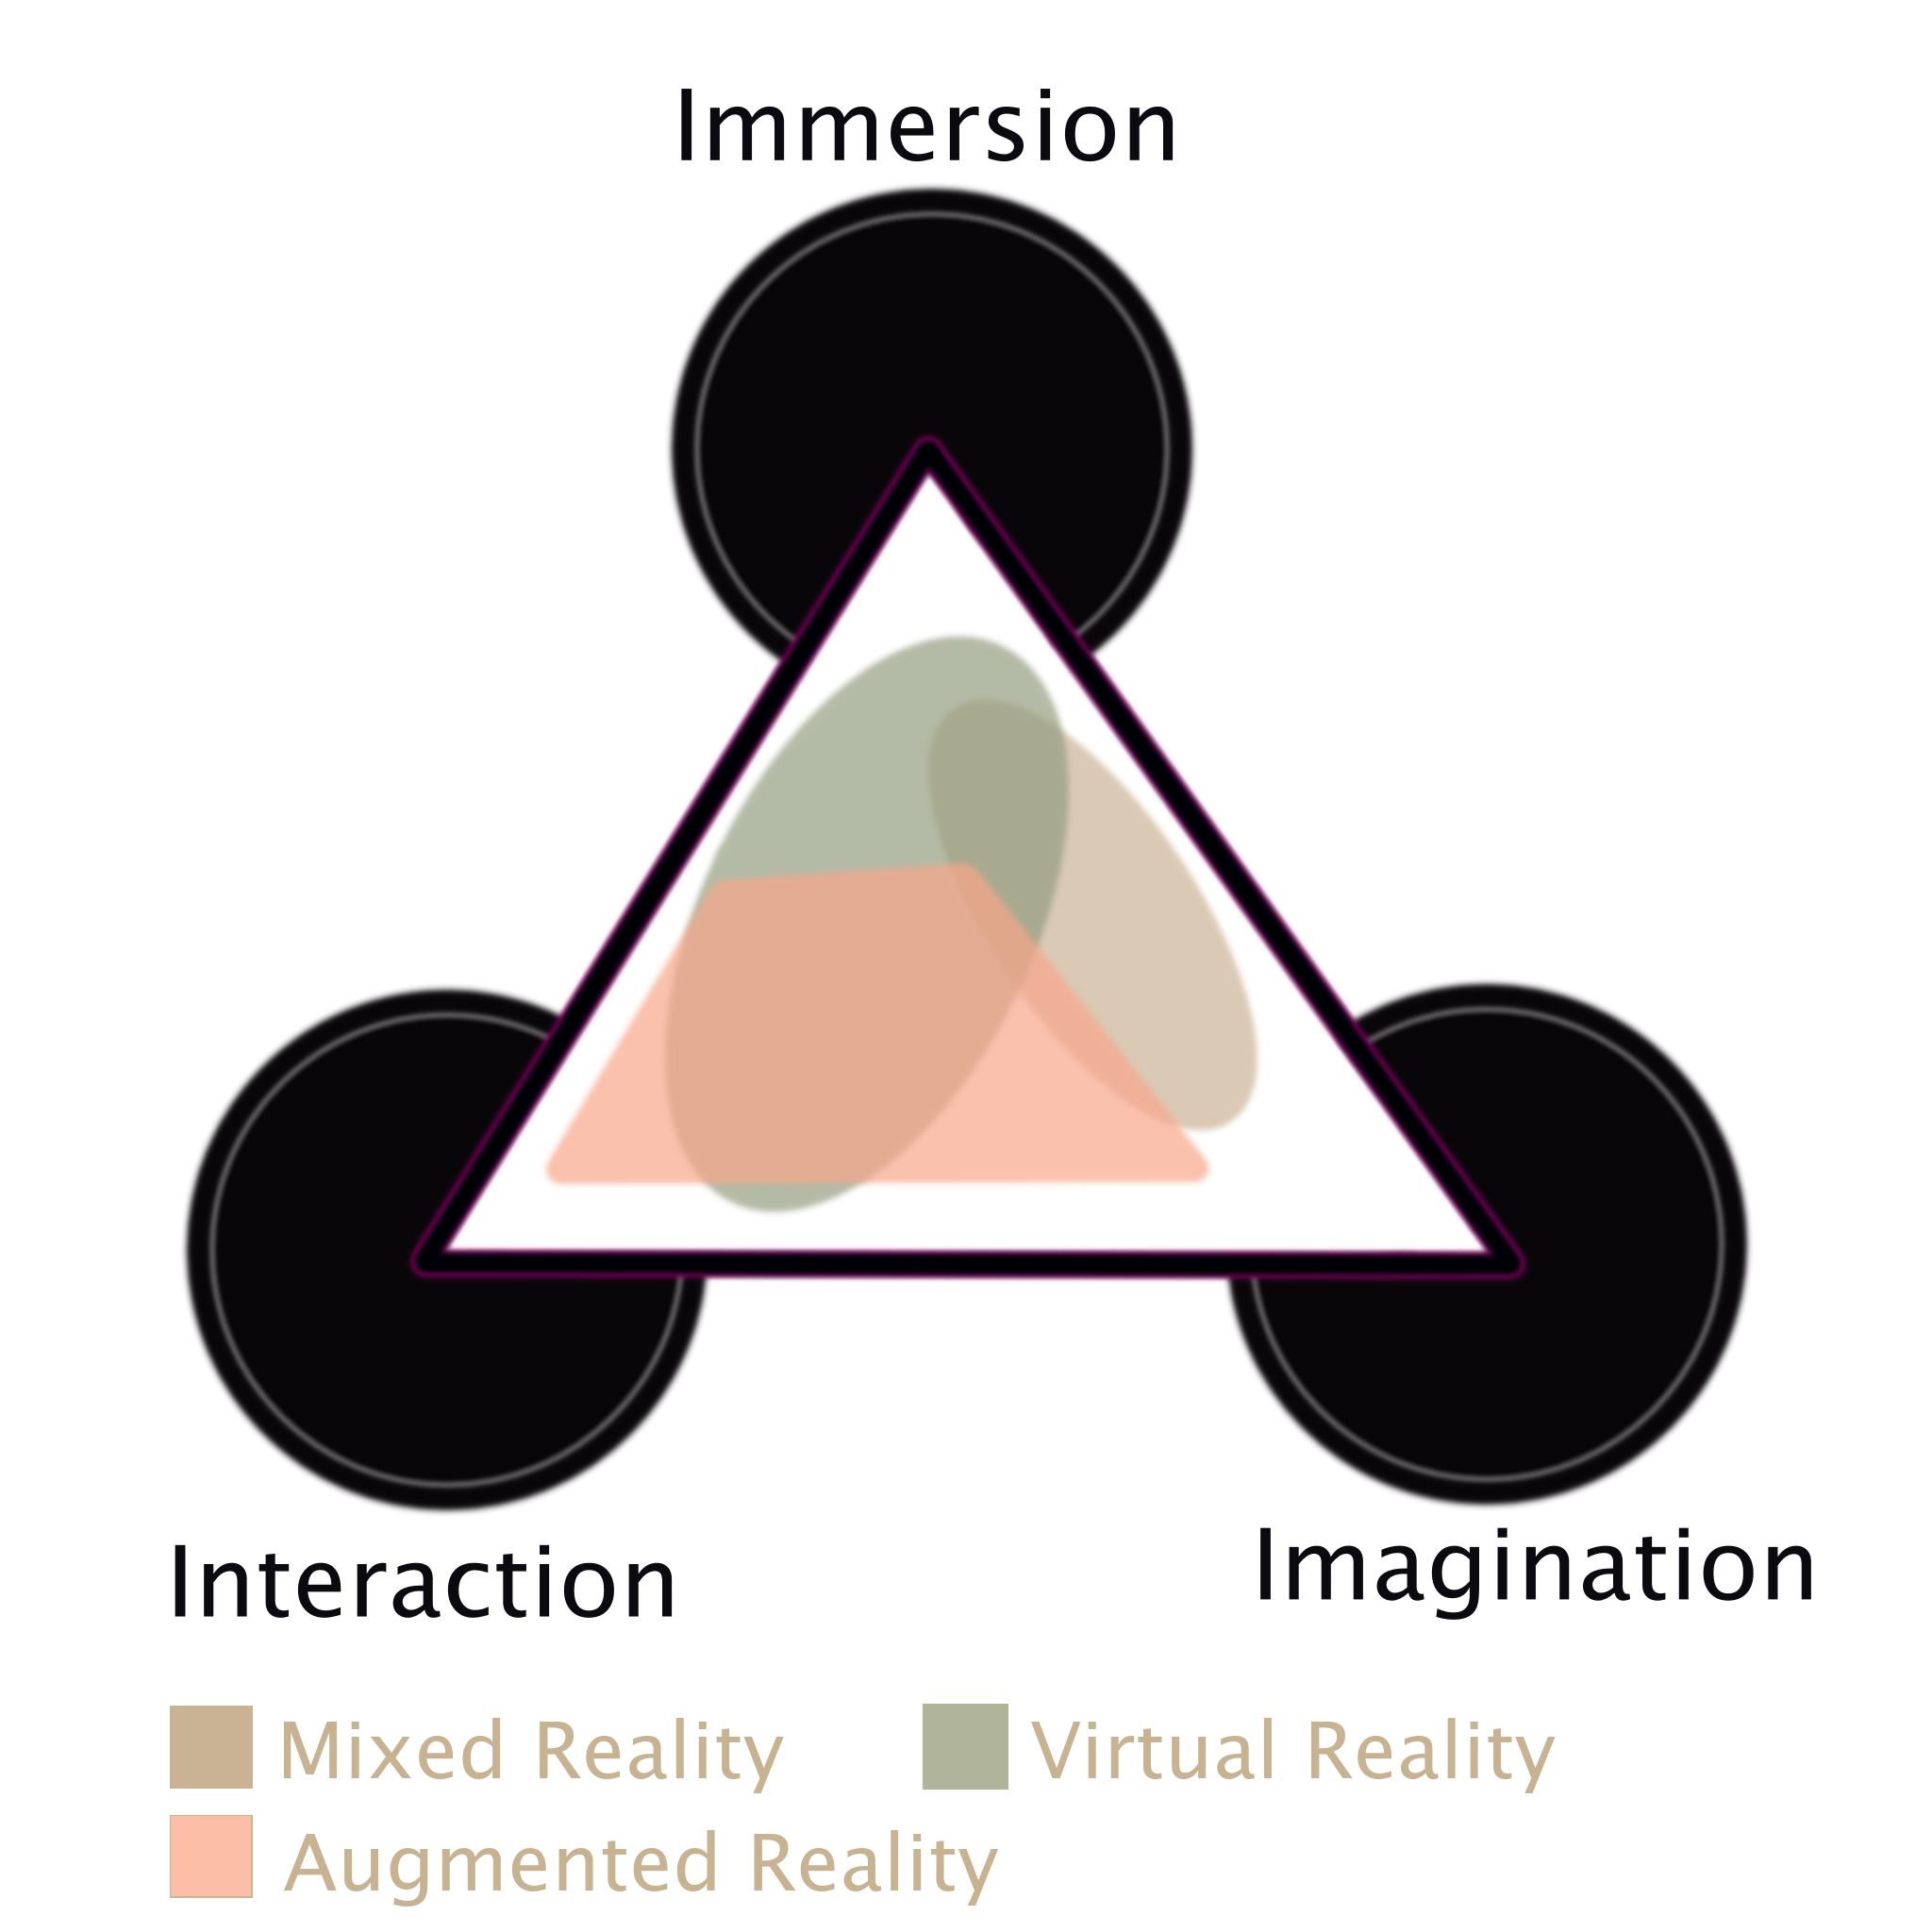
\includegraphics[width=\textwidth]{_raw_resources/i3-triangle.png}
	\caption{I\textsuperscript{3} Triangle - figurative quantization of 
		different reality extending methods}
	\label{fig:xr:i3-triangle}
\end{figure}
Augmented Reality (AR) is a concept by augmenting real world imagery with 
additional information and interactable objects. It used to be called Mixed 
Reality\cite{satoh:case:1998} \cite{tamura:mixed-reality:2001}, merging real 
world imagery with 3D objects but has slowly adapted to AR, since they both 
described the same concept. It ranges from very simple devices displaying data 
in the field of view of an user up to full augmentation, displaying 3D models 
overlaying on real world objects. This can be done ranging from Pepper's Ghost 
projections, augmenting video - a famous example is the rather successful 
"Pokémon GO" -, up to the Microsoft HoloLens, that has sensors for a wide range 
of spatial mapping, spatial anchoring and distant field calculation.

Virtual Reality is a concept usually done by stereo projection of a 3D 
environment inside a Head Mounted Display. It takes an user out of the current 
room and sets him into a complete new, virtual reality - hence its names 
origin. HMD hardware ranges from the simplistic Google Cardboard 
\footnote{using a smart phone as display device} to the Samsung GearVR 
\footnote{similarly uses a smart phone as display driver} up to the Oculus Rift 
and HTC Vive\footnote{which are driven by a mid- to high range PC}. The latter 
two products offer room-scale experiences where an user is able to move freely 
in his play space (basically a tacked bounding volume) and allows for six 
degrees of freedom (\gls{6dof}) tracking.

Mixed Reality is an extension of Virtual Reality, allowing bystanders to get an 
impression of the virtual 3D environment around an actor. By reproducing 
virtual projection parameters of a 3D environment, it is possible to place a 
real world camera feed at the right position inside the 3D scene. This 
yields a combined application of Augmented and Virtual Reality technique. A 
production environment can be achieved with a \gls{6DOF} HMD and additional - 
either user or tracking input for positional and rotational parameters for the 
real world camera. 

\section{Immersion vs. Communication}

\todo[inline]{maybe the overview does already a "good enough" job to bring this 
across.}

Virtual Reality, as previously mentioned in \ref{sec:intro:outline}, is very 
immersive but the experience is hard to imagine without wearing a HMD yourself. 
Additionally doesn't VR offer any ways to allow observers a similar experience 
as the VR actor.
\newline
A very obvious problem starts on interaction. A VR user doesn't always need to 
see his hands to interact with a scene due to the natural way of holding these 
controllers in his hands and directly translating controller interaction to the
virtual environment. However an outside viewer does not see the actors hands 
and will not understand any actions performed by the user if he doesn't see the 
virtual hands. Any usage context that happens off-screen cannot be communicated 
and therefore will be lost.
\newline
A recent game example, Rick and Morty: Virtual Rick-ality, tries to mitigate 
this issue by placing virtual CCTV cameras into the scene, which can be 
controlled through outside observers - giving a neutral third-person view into 
the three-dimensional scene. A VR actor is replaced as a loose avatar 
representing a figure (Morty) from the cartoons universe.
\todo{Add a screenshot of that}

Mixed Reality merges the actors and virtual realities context, allowing outside 
bystanders a comparable window into the actors experienced world. In fact, 
initial promotional material for the HTC Vive showed mixed reality footage, 
produced by one VR computer and a secondary composition PC 
\cite{valve:mr-production:2016}. It's setup is comparable to the one in this 
thesis and differs by composition techniques and by using more than one 
software context, done by outputting a rendered image of the virtual scene and 
compositing it on another system.

\subsection{Evolution of Virtual Reality Footage}

Originally VR footage consisted of the output that was sent to the headset, 
including image transformation that needs to be done to correct the headset 
lenses \footnote{this is referred to as "Barrel Distortion"} - this distorted 
dual image is very hard to follow, as it adds two ambiguous images and has 
additional a high distortion. Since the direct feed to a HMD is used, any 
translation of the headsets position is visible, which results in a jittery and 
unnatural looking motion feed.

\begin{figure}[htbp]
	\label{fig:evolution:steps}
	\begin{subfigure}[t]{.45\textwidth}
		\centering
		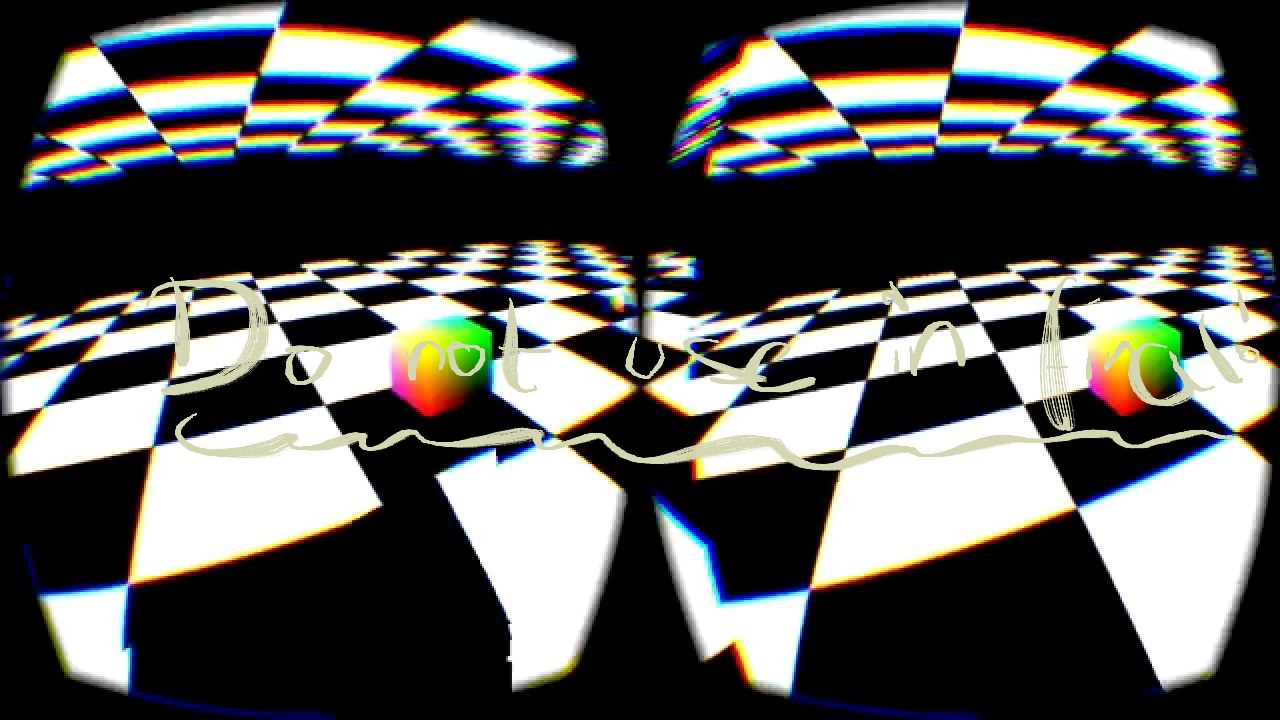
\includegraphics[width=\textwidth]{_raw_resources/lens_distortion.jpeg}
		\caption{Distorted direct dual output to a Oculus DK2.}
	\end{subfigure}
	\begin{subfigure}[t]{.45\textwidth}
		\centering
		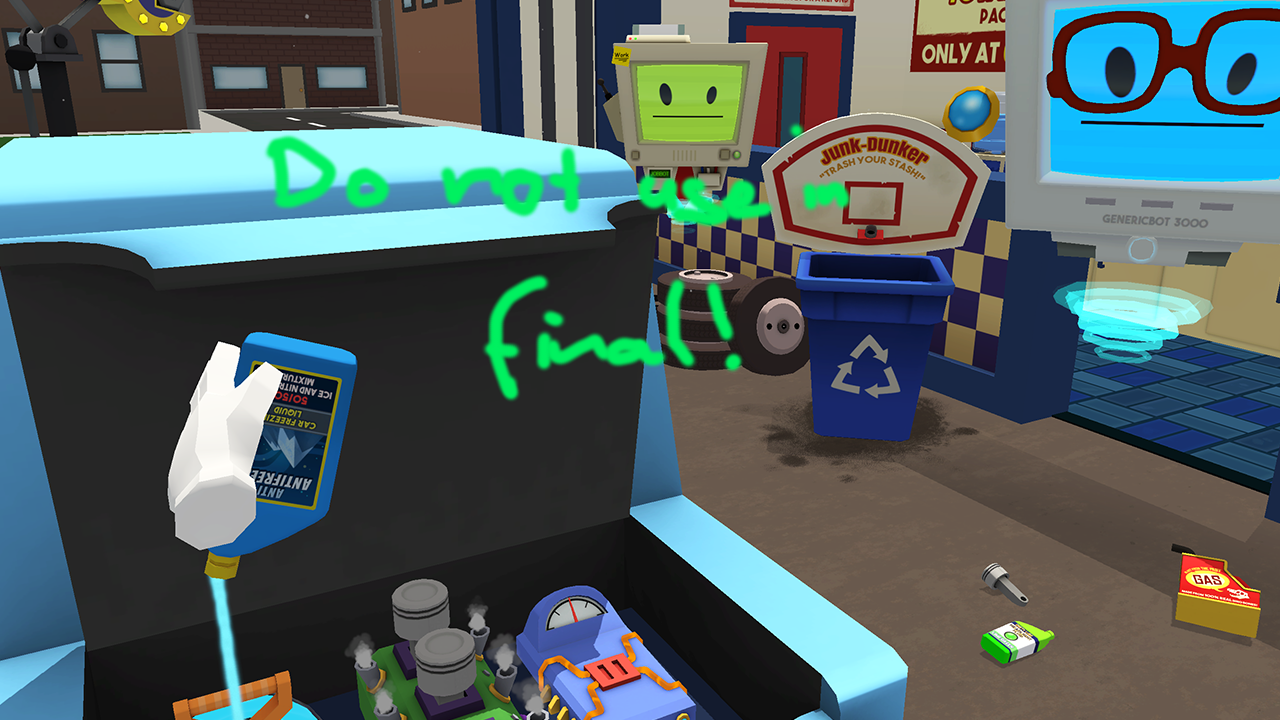
\includegraphics[width=\textwidth]{_raw_resources/job_simulator_vr.png}
		\caption{A first person, single screen output is an improvement, but is 
			hard to follow in motion.}
	\end{subfigure}
	\newline
	\begin{subfigure}[t]{.45\textwidth}
		\centering
		
\includegraphics[width=\textwidth]{_raw_resources/rickality_cctv.png}
		\caption{"Rick and Morty: Virtual Rick-Ality" allows outside observers 
			to control mounted CCTV cameras to observe the actors interaction.}
	\end{subfigure}
	\begin{subfigure}[t]{.45\textwidth}
		\centering
		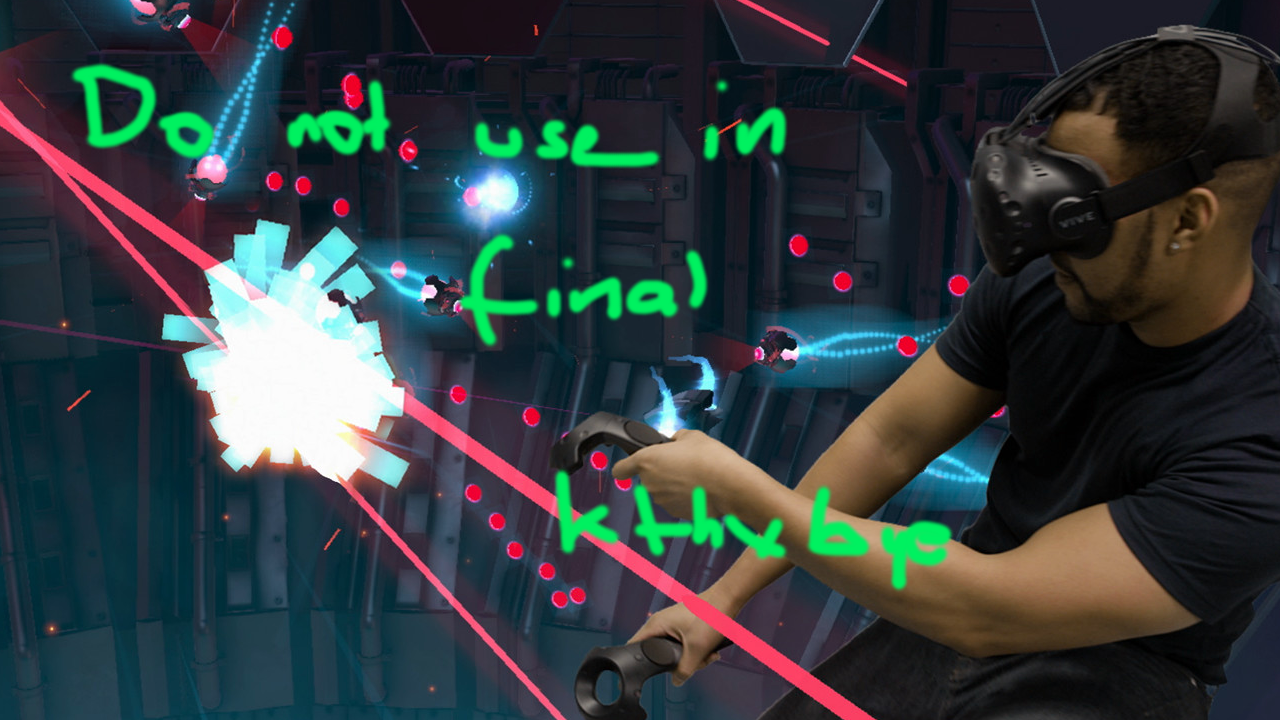
\includegraphics[width=\textwidth]{_raw_resources/the_lab_mr.png}
		\caption{Currently a screenshot of The Lab MR - but actually will be 
			one of my solution. Just gotta take some screenshots.}
	\end{subfigure}
\end{figure}

A next step was to render one eye in fullscreen of the attached monitor and do 
all image transformations (mainly crop and distort) after rendering it, 
allowing bystanders to get a clear first person image of the actors experience. 
Additionally, as a secondary camera, a dampened movement can be set to mitigate 
jittery motion. As previously pointed out, this works but sometimes loses 
interaction context, especially when no hands are visible. 
\newline
Then there is currently only one game, Rick and Morty: Virtual Rick-ality, that 
has an optional CCTV feature enabled, in which third persons can control a 
variety of mounted, virtual cameras and follow the actors interaction with the 
3D environment. This VR actor is then replaced with an avatar to visualize what 
how he is interacting with the scenery.
\todo{Maybe I should pin down the timeline - how long it took for a 
next step to emerge from the medium.}
\newline
Finally there is mixed reality, where the VR actor is placed in context of 
the virtual reality scene. This has been done previously by post-production for 
trailers and allows for a better understanding between virtual interaction and 
real actor motion. With its help it is possible to invite third person viewers 
into the VR experience in a natural way.

\section{Mixed Reality and its use cases}

\todo{There is a meeting planned to discuss A+Cs interest and use cases 
for MR - which then probably ends up in here in a summary.}

\section{Current state of Mixed Reality Production}

There have been an increasing number of presentations for mixed reality setups. 
To sort this thesis into the current scope of production environments, it is 
necessary to look at other approaches and their differences to the proposed 
solution.

\subsection{SteamVR \& Oculus SDK plugins}

Both SteamVR and Oculus SDKs supply plugins to enable mixed reality capturing. 
These system approach the problem similarly by compositing an incoming video 
stream directly at the current position of an registered camera tracker, thus 
failing to accommodate for different input latencies from the motion video 
feed, yielding an inconsistent visual performance. Oculus states on their 
manuals, that these are currently only intended "for proof-of-concept, 
troubleshooting, and hobby use." \ref{oculus:mr-setup:2017}
\newline
In addition SteamVRs solution supports only video-output composition with a 4K 
HDMI output - which in turn means that the signal has to be captured on an 
external device and has to be composited on a secondary system. The 
configuration parameters are "barebones" at best and yielding good results is a 
matter of the best possible studio setup capture.

\subsection{Fantastic Contraption}

The game "Fantastic Contraption" from 2016 allows livestreamers to do a video 
composition for mixed reality. While this approach allows to mitigate video 
input delays it cannot have a free moving camera with an additional motion 
tracker.
\newline
"Fantastic Contraptions" trailers also show another approach by replacing the 
actor with an avatar by basically rendering a certain depth and then placing 
real world camera footage as background. With such a system any live video 
background removal is not necessary and real world footage of the actor is 
lost. The games trailer composition has been achieved in post production. 
\cite{gartner:cinematography:2017}

\subsection{Owlchemy Labs Mixed Reality}

Owlchemy Labs is a VR game developer located in Austin, Texas. They're working 
on VR experiments and use similar techniques discussed in this paper. Their key 
difference in visual reproduction is by using a stereoscopic camera to record 
an actor and can reproduce the actors depth per pixel, allowing for more 
complex fore- and background separation for a more accurate visual reproduction.
\newline
While Owlchemy Labs announced real time mixed reality compositing, there hasn't 
been a shipped product or update for one of their games that allows for live 
mixed reality capture. \todo{Sauce!11!}

\subsection{Apple Keynote}

Apple presented a real time mixed reality showcase done on their computer 
systems on their annual keynote "WWDC17". It is driven by Unreal Engine and 
uses also similar techniques as discussed in this thesis. That presentation is 
currently the best live performance of mixed reality with a high quality chroma 
keying, depth reconstruction and high fidelity graphics. There is no technical 
information available yet. \todo{Gimme that sauce, at least 'ze video!}
% !TeX spellcheck = en_US
% !TEX root = ../thesis-example.tex
%
\chapter{System Setup}
\label{ch:system-setup}

The following section describes the hard- and software components used for the 
thesis and results. All demonstrations have been performed on that environment. 
All dependencies have been explicitly marked to allow a similar, but not exact, 
setup to reproduce these results.

\begin{figure}[htb]
	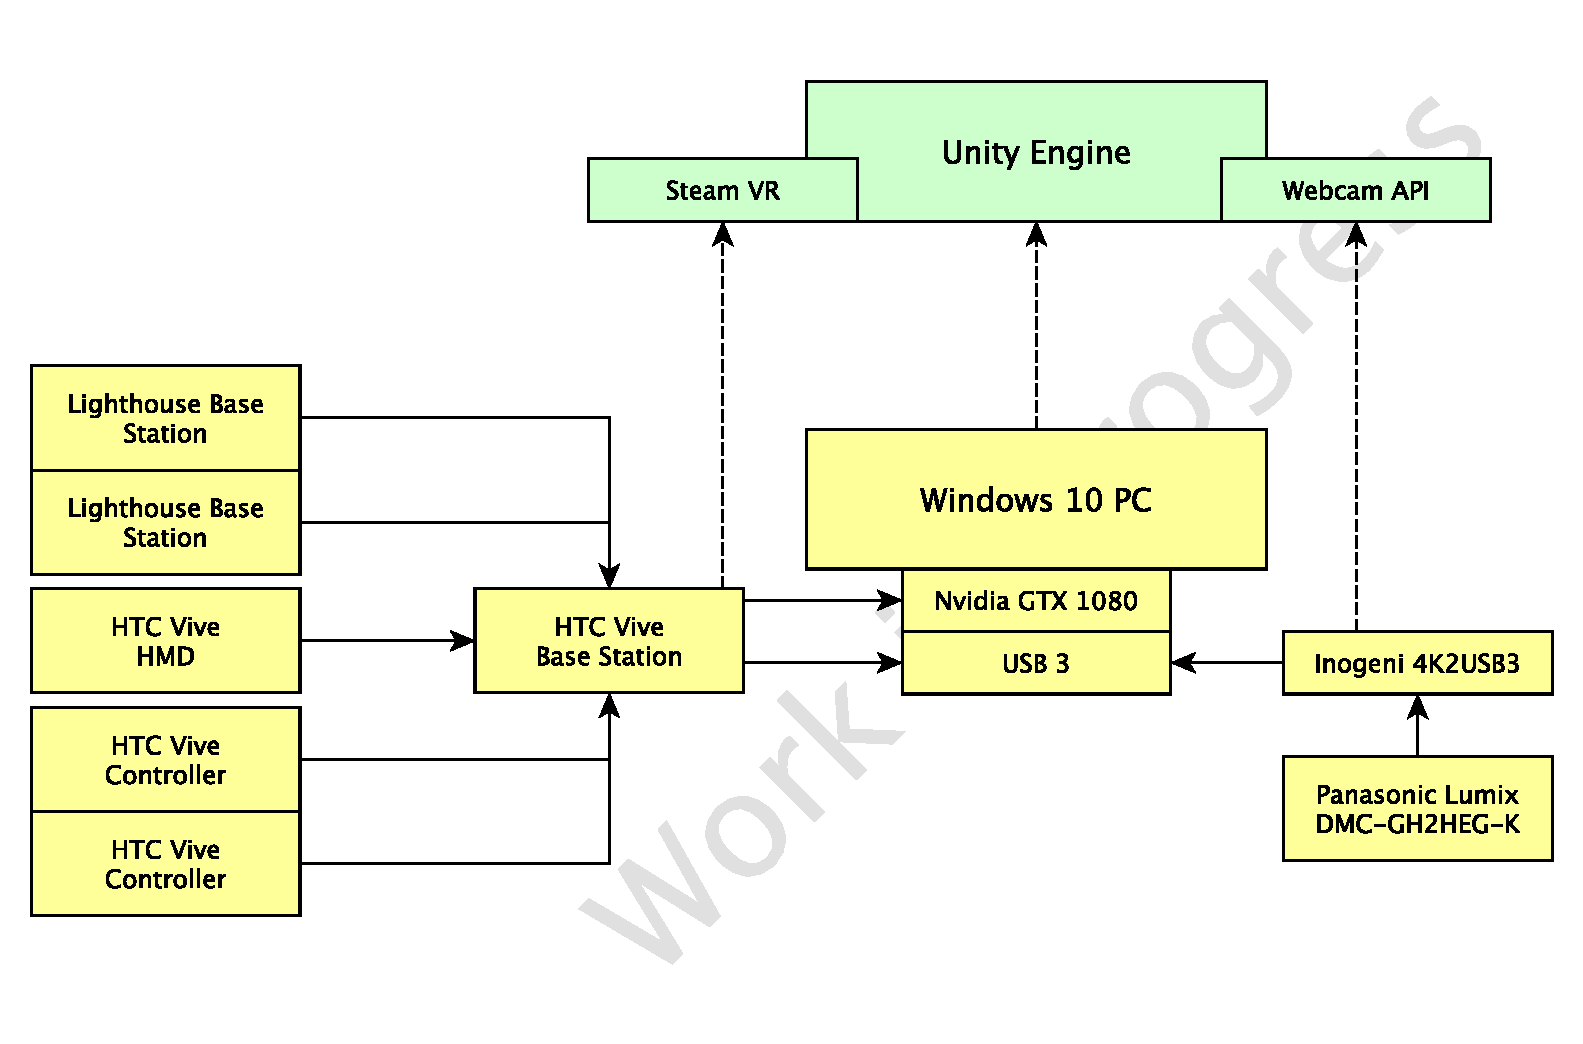
\includegraphics[width=\textwidth]{gfx/System-Components}
	\caption{Diagram of hard- and software components.}
	\label{fig:system-components}
\end{figure}

\section{Hardware Configuration}
\label{sec:hardware-config}

The hardware configuration is split in three main parts:
\begin{my_list}
	\item Windows PC Workstation
	\item Virtual Reality Tracking Solution
	\item Motion Video Input Feed
\end{my_list}

Each individual configuration is basically interchangeable with other systems, 
as long as predefined conditions are met. Each condition is listed first in 
each subsection.

\subsection{PC Workstation}

As the software is built in the Unity Engine, the workstation is limited to 
either Windows or Mac OS X systems the only requirement - besides being 
powerful enough to render the 3D scenes - is two USB3 ports to ensure enough 
data throughput for the video and virtual reality solution, as well as two 
video outputs for a monitor and its headset.
\newline
The configuration used for this thesis is:
\begin{lstlisting}
	CPU: Intel i7-6700 @ 3.40 GHz
	RAM: 16GB DDR4
	GPU: Nvidia Geforce GTX 1080
	System: Windows 10 v. 1703
	Engine: Unity 5.6f3
\end{lstlisting}

This system configuration is to date a high-end workstation that has an 
abundance of render performance and memory for complex and taxing computations 
that have to be performed for a mixed reality composition.

\subsection{Inogeni 4K2USB3 Capture Device}
The Ingoeni 4K2USB3 converter is a standalone box that allows to receive any 
HDMI source and converts it as a webcam video feed usable by "plug'n'play" 
device management of Windows. It's advantage is that it enables any HMDI source 
to be usable as system webcam, thus enabling and arbitrary choice of video 
cameras and a very simple integration with any software through the systems 
provided webcam API. With help of the converter box it's possible to request a 
webcam as video resource and process that video feed as a texture on the GPU.

\subsection{Panasonic GH2 System Camera}
This camera provides a direct video feed via HDMI with low latency. It can 
directly feed into the Inogeni 4K2USB3 and produces a stable, high quality 
video feed with a low signal to noise ratio in well lit environments. 
Additionally it has a well sized photo sensor allowing the camera to capture 
singular frames with reduced motion blur.

\subsection{HTC Vive with Controllers and Lighthouses}
The currently best virtual reality and tracking device available to the public 
is the HTC Vive. It includes two infrared sending stations called "Lighthouse", 
two Vive Controllers\footnote{often delightfully called "Wands" due to its 
controllers design} and a headset. Both, headset and controller systems, are 
enabled with 6 degrees of freedom (6DOF) tracking. The tracking system is a 
black box, in which only the transformation matrices for the hand controllers 
and the HMD can be accessed\footnote{as well as sensor input data from the 
controllers}, which already have been processed by the additional SteamVR 
software. By default this transformation has a normalized length of 1 unit to 1 
meter. Designing scenery and sense of size is therefore rather imaginable. The 
data provisioning is done by a library called "SteamVR for Unity", which makes 
the usage of said matrices in engine fully transparent.

\subsection{Vive Controller Tripod Mount}
Most cameras have a standardized way of mounting tripods. Since the Vive  
controllers have no reference plane. Minuscule differences in mounting angles 
change the projection parameters to noticeable effects, so it was necessary to 
build a mount for the camera to keep controller and video equipment 
transformation synchronized.

\begin{figure}[htb]
	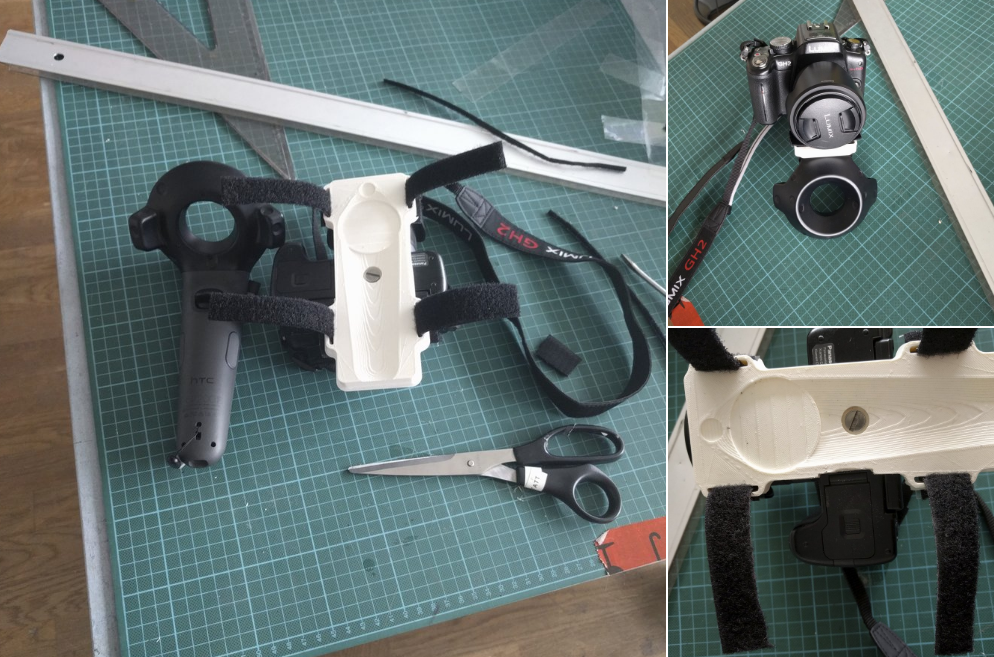
\includegraphics[width=\textwidth]{_raw_resources/ViveStrap-Mount.png}
	\caption{Camera mount for a HTC Vive controller, mounted on the cameras 
		tripod mount}
	\label{fig:system:camera-mount}
\end{figure}

I've built a mount that fits on tripod attachment points and keeps the 
controller locked in the same rotation and position (see figure 
\ref{fig:system:camera-mount}).



\section{Software}

The software of choice is Unity3D, which is a free game engine for students, 
non-profit organizations and small studios. It provides an easy introduction to 
game / 3D engine programming and has a huge development community. While it is 
not the technologically most advanced engine, its fairly easy usage and fast 
development cycles make it a great tool for a bachelor thesis.
\newline
Thankfully, the high abstraction of system APIs means that cross-platform 
development only needs a single code base and makes excruciating tasks like 
webcam access simple - so much so that it boils down to one line of code. 
However, this has drawbacks in overall performance, partially introduced by the 
engine's garbage collection, which are no issue for the used system.
\newline
Its weakness is usually API documentation and - on the downside, too - high 
abstraction levels from most APIs. For example, Unity relies on its own shading 
language which cross-compiles to HLSL, OpenGL and WebGL - this leads to 
problems in buffer and data management, which cannot be controlled well inside 
its render loop.

The software discussed in this thesis integrates and depends additionally on 
SteamVR, a library for Unity, providing the necessary tracking data in the 
engine. SteamVR is developed by Valve, the software is available for free on 
Steam, the complementary library is hosted on GitHub. As of writing this 
thesis, SteamVR is available for Windows and Mac OS X and the software of this 
thesis works on both systems. 

There are no further dependencies or external libraries used.
% % !TEX root = ../thesis-example.tex
%
\chapter{Concepts: This text is here to test a very long title, to simulate the line break behavior, to show that an extremely long tilte also works}
\label{sec:concepts}

\cleanchapterquote{Users do not care about what is inside the box, as long as the box does what they need done.}{Jef Raskin}{about Human Computer Interfaces}

\Blindtext[2][1]

\section{Concepts Section 1}
\label{sec:concepts:sec1}

\Blindtext[2][2]

\section{Concepts Section 2}
\label{sec:concepts:sec2}

\Blindtext[3][2]

\section{Concepts Section 3}
\label{sec:concepts:sec3}

\Blindtext[4][2]

\section{Conclusion}
\label{sec:concepts:conclusion}

\Blindtext[2][1]
 % INCLUDE: concepts
% % !TEX root = ../thesis-example.tex
%
\chapter{Conclusion}

\subsection{3D Environment and Composition Considerations}
\subsection{Performance Considerations} % INCLUDE: conclusion
\cleardoublepage

% --------------------------
% Back matter
% --------------------------
{%
\setstretch{1.1}
\renewcommand{\bibfont}{\normalfont\small}
\setlength{\biblabelsep}{0pt}
\setlength{\bibitemsep}{0.5\baselineskip plus 0.5\baselineskip}
\printbibliography[nottype=online]
\printbibliography[heading=subbibliography,title={Websites},type=online,prefixnumbers={@}]
}
\cleardoublepage

\listoffigures
\cleardoublepage

\listoftables
\cleardoublepage

% !TEX root = ../thesis-example.tex
%
\pagestyle{empty}
\hfill
\vfill
\pdfbookmark[0]{Colophon}{Colophon}
\section*{Colophon}

This thesis was typeset with \LaTeXe.
It uses the \textit{Clean Thesis} style developed by Ricardo Langner.
The design of the \textit{Clean Thesis} style is inspired by user guide documents from Apple Inc.

Download the \textit{Clean Thesis} style at \url{http://cleanthesis.der-ric.de/}.

\cleardoublepage

% !TEX root = ../thesis-example.tex
%
%************************************************
% Declaration
%************************************************
\pdfbookmark[0]{Declaration}{Declaration}
\chapter*{Declaration}
\label{sec:declaration}
\thispagestyle{empty}

Hereby I affirm that this thesis is written by myself and I have not used any 
additional resources or utilities.

\begin{center}
	\hrulefill
\end{center}

Ich versichere, dass ich meine Abschlussarbeit selbstständig verfasst und keine 
anderen als die angegebenen Quellen und Hilfsmittel benutzt habe.

\bigskip

\noindent\textit{\thesisUniversityCity, \thesisDate}

\smallskip

\begin{flushright}
	\begin{minipage}{5cm}
		\rule{\textwidth}{1pt}
		\centering\thesisName, Matr.-Nr. 824320
	\end{minipage}
\end{flushright}

%*****************************************
%*****************************************

\clearpage
\newpage
\mbox{}

% **************************************************
% End of Document CONTENT
% **************************************************
\end{document}
